\documentclass[14pt,a4paper]{extarticle}

% --- 1. Поддержка кириллицы, кодировок и шрифтов (СТП 01-2017) ---
\usepackage{cmap}
\usepackage[T2A]{fontenc}
\usepackage[utf8]{inputenc}
\usepackage[russian]{babel}
\usepackage{tempora} % Истинный Times New Roman для кириллицы и латиницы (с полной поддержкой Bold/Italic)

% --- 2. Геометрия страницы по СТП 01-2017 и образцу ОтчетRest.docx (Левое 30мм, Правое 15мм, Верхнее 20мм, Нижнее 20мм) ---
\usepackage[a4paper, left=30mm, right=15mm, top=20mm, bottom=20mm]{geometry}

% --- 3. Межстрочный интервал (полуторный) и абзацный отступ (1.25 см) ---
\usepackage{setspace}
\setstretch{1.25}
\usepackage{indentfirst}
\setlength{\parindent}{1.25cm}
\setlength{\parskip}{0pt}

% --- 4. Предотвращение выезда длинных слов и идентификаторов за границы листа ---
\sloppy
\emergencystretch=2.5em
\righthyphenmin=2
\lefthyphenmin=2

% --- 5. Математические пакеты и таблицы ---
\usepackage{amsmath,amssymb}
\usepackage{array}
\usepackage{tabularx}
\usepackage{booktabs}
\usepackage{graphicx}
\usepackage{float}
\usepackage{caption}

% --- 6. Оформление подписей к рисункам и таблицам по СТП 01-2017 (длинное тире) ---
\DeclareCaptionLabelSeparator{emdash}{~---~}
\captionsetup[figure]{name=Рисунок, labelsep=emdash, justification=centering, font=normalfont, size=normalsize}
\captionsetup[table]{name=Таблица, labelsep=emdash, justification=raggedright, singlelinecheck=false, font=normalfont, size=normalsize}

% --- 7. Оформление заголовков разделов и подразделов по СТП 01-2017 (14pt, абзацный отступ 1.25 см) ---
\usepackage{titlesec}
\titleformat{\section}[block]{\bfseries\normalsize\raggedright}{\thesection}{1em}{\MakeUppercase}
\titleformat{\subsection}[block]{\bfseries\normalsize\raggedright}{\thesubsection}{1em}{}
\titleformat{\subsubsection}[block]{\bfseries\normalsize\raggedright}{\thesubsubsection}{1em}{}

\titlespacing*{\section}{\parindent}{18pt}{18pt}
\titlespacing*{\subsection}{\parindent}{18pt}{18pt}
\titlespacing*{\subsubsection}{\parindent}{18pt}{18pt}

% --- 8. Листинги кода по СТП 01-2017 (без номеров строк слева, с рамкой и переносом) ---
\usepackage{fvextra}
\usepackage{fancyvrb}
\DefineVerbatimEnvironment{CodeListing}{Verbatim}{
    fontsize=\fontsize{9.5pt}{11.5pt}\selectfont,
    frame=single,
    framesep=2.5mm,
    framerule=0.5pt,
    breaklines=true,
    breaksymbol={\tiny\ensuremath{\hookrightarrow}},
    xleftmargin=0pt,
    xrightmargin=0pt
}

% --- 9. Списки: отступы и стиль маркированных списков (маркер-дефис -) ---
\usepackage{enumitem}
\setlist{nosep, leftmargin=1.25cm}
\setlist[enumerate]{label=\arabic*., leftmargin=1.25cm}
\setlist[enumerate,1]{label=\arabic*., leftmargin=1.25cm}
\setlist[enumerate,2]{label=\arabic{enumi}.\arabic*., leftmargin=1.25cm}
\setlist[itemize]{label=-, leftmargin=1.25cm}
\renewcommand{\labelitemi}{-}
\renewcommand{\labelitemii}{-}

% --- 10. Нумерация страниц справа по СТП 01-2017 ---
\usepackage{fancyhdr}
\pagestyle{fancy}
\fancyhf{}
\fancyfoot[R]{\thepage}
\renewcommand{\headrulewidth}{0pt}
\renewcommand{\footrulewidth}{0pt}

\fancypagestyle{plain}{
    \fancyhf{}
    \fancyfoot[R]{\thepage}
    \renewcommand{\headrulewidth}{0pt}
    \renewcommand{\footrulewidth}{0pt}
}

\usepackage{hyperref}
\hypersetup{
    colorlinks=true,
    linkcolor=black,
    citecolor=black,
    filecolor=black,
    urlcolor=blue
}

\begin{document}

% ==============================================================================
% ТИТУЛЬНЫЙ ЛИСТ (образцу СТП 01-2017 и ЛР1, без слова вариант)
% ==============================================================================
\begin{titlepage}
    \begin{center}
        Министерство образования Республики Беларусь\\[0.15cm]
        Учреждение образования\\[0.15cm]
        «БЕЛОРУССКИЙ ГОСУДАРСТВЕННЫЙ УНИВЕРСИТЕТ\\
        ИНФОРМАТИКИ И РАДИОЭЛЕКТРОНИКИ»
    \end{center}
    
    \vspace{0.4cm}
    
    \begin{flushleft}
        Факультет компьютерных систем и сетей\\[0.1cm]
        Кафедра программного обеспечения информационных технологий\\[0.1cm]
        Дисциплина: Методы машинного обучения (ММО)
    \end{flushleft}
    
    \vspace{2.2cm}
    
    \begin{center}
        \large\textbf{ОТЧЕТ}\\[0.2cm]
        \normalsize
        {по лабораторной работе № 3}\\[0.3cm]
        Тема работы: Градиентный спуск, стохастический градиентный спуск и регуляризация
    \end{center}
    
    \vspace{2.5cm}
    
    \noindent
    \begin{tabular}{@{}p{0.62\textwidth}@{}p{0.38\textwidth}@{}}
        Выполнила: & \\
        студентка гр. 351002 & Алексейчик Я.\,Н. \\[0.5cm]
        Проверил: & Лебедевич А.\,В.
    \end{tabular}
    
    \vfill
    
    \begin{center}
        Минск 2026
    \end{center}
\end{titlepage}

\setcounter{page}{2}

% ==============================================================================
\section{Цель работы}
% ==============================================================================
Изучение математических основ и практическая программная реализация методов оптимизации функционалов качества в задачах линейной регрессии:
\begin{enumerate}
    \item Реализация алгоритма пакетного градиентного спуска (Batch Gradient Descent) с векторным расчетом градиентов и критерием останова по евклидовой норме изменения весов $\|w^k - w^{k-1}\|_2 < \varepsilon$;
    \item Экспериментальное исследование влияния шага обучения (Learning Rate $\eta$) на скорость сходимости и устойчивость алгоритма;
    \item Реализация стохастического градиентного спуска (Stochastic Gradient Descent) со случайным выбором объектов и расписанием затухания темпа обучения Роббинса-Монро;
    \item Сравнительный анализ скорости сходимости GD и SGD на одном графическом поле;
    \item Реализация $L_1$-регуляризации (Lasso) для четного варианта 2 через проксимальный оператор Soft-Thresholding (ISTA), а также $L_2$-регуляризации (Ridge) для 20 значений параметра $\lambda$ в диапазоне от $0.001$ до $1000$;
    \item Сравнение полученных параметров с библиотечными реализациями Scikit-Learn.
\end{enumerate}

% ==============================================================================
\section{Описание набора данных и предварительная обработка}
% ==============================================================================
В качестве предметной базы использован набор данных из Лабораторной работы №2 (\texttt{StudentPerformanceFactors.csv}, $N = 6607$ наблюдений).

Для выполнения условия задания «не менее 2 признаков без учета целевого (не менее 3 весов)» сформирован набор из $m=6$ физически интерпретируемых признаков, что с учетом фиктивного единичного столбца для свободного члена $w_0$ образует вектор из 7 весовых параметров:
\begin{itemize}
    \item \texttt{Hours\_Studied} --- количество часов самостоятельных занятий в неделю;
    \item \texttt{Attendance} --- посещаемость учебных занятий (\%);
    \item \texttt{Previous\_Scores} --- результаты предварительного тестирования;
    \item \texttt{Tutoring\_Sessions} --- число индивидуальных занятий с репетитором;
    \item \texttt{Physical\_Activity} --- часы физической культуры и спорта;
    \item \texttt{Parental\_Involvement} --- степень вовлеченности родителей в образовательный процесс.
\end{itemize}
Целевая переменная: \texttt{Exam\_Score} --- итоговая экзаменационная оценка студента (баллы от 0 до 100).

\textbf{Предотвращение утечки данных (Data Leakage):}  
Масштабирование признаков алгоритмом \texttt{StandardScaler} ($z = \frac{x - \mu}{\sigma}$) обучено строго на обучающей подвыборке ($80\%$, $N_{train} = 5285$), после чего применилось к тестовой подвыборке ($20\%$, $N_{test} = 1322$). Признак \texttt{Score\_Improvement} исключен, так как он содержит целевую переменную.

% ==============================================================================
\section{Математические основы алгоритмов оптимизации}
% ==============================================================================

\subsection{Пакетный градиентный спуск (BGD)}
Функция потерь среднеквадратичной ошибки (MSE):
\begin{equation}
    Q(w) = \frac{1}{n} \sum_{i=1}^n (\hat{y}_i - y_i)^2 = \frac{1}{n} \|X_b w - y\|_2^2
\end{equation}
Векторный градиент по весам $w \in \mathbb{R}^{m+1}$:
\begin{equation}
    \nabla Q(w) = \frac{2}{n} X_b^T (X_b w - y)
\end{equation}
Правило обновления весов:
\begin{equation}
    w^k = w^{k-1} - \eta \cdot \frac{2}{n} X_b^T (X_b w^{k-1} - y)
\end{equation}
Критерий останова итерационного процесса:
\begin{equation}
    \|w^k - w^{k-1}\|_2 = \sqrt{\sum_{j=0}^m (w_j^k - w_j^{k-1})^2} < \varepsilon = 10^{-6}
\end{equation}

\subsection{Стохастический градиентный спуск (SGD)}
На шаге $k$ выбирается случайный индекс объекта $i \in \{0, \dots, n-1\}$. Стохастический градиент:
\begin{equation}
    \nabla q_i(w^{k-1}) = 2 (x_i^T w^{k-1} - y_i) x_i
\end{equation}
Расписание скорости обучения для гарантированной сходимости по условию Роббинса-Монро ($\sum \eta_k = \infty, \sum \eta_k^2 < \infty$):
\begin{equation}
    \eta_k = \frac{\eta_0}{1 + \alpha \cdot k}, \quad \eta_0 = 0.01, \quad \alpha = 0.0001
\end{equation}

\subsection{L1-регуляризация (Lasso, Вариант 2)}
Минимизируемый функционал (смещение $w_0$ не штрафуется):
\begin{equation}
    Q_{L1}(w) = \frac{1}{n} \|X_b w - y\|_2^2 + \lambda \sum_{j=1}^m |w_j|
\end{equation}
Проксимальный шаг Soft-Thresholding (ISTA):
\begin{equation}
    \tilde{w} = w^{k-1} - \eta \nabla Q(w^{k-1})
\end{equation}
\begin{equation}
    w_0^k = \tilde{w}_0, \quad w_j^k = \text{sign}(\tilde{w}_j) \cdot \max(0, |\tilde{w}_j| - \eta \lambda), \quad j = 1, \dots, m
\end{equation}

\subsection{L2-регуляризация (Ridge)}
\begin{equation}
    Q_{L2}(w) = \frac{1}{n} \|X_b w - y\|_2^2 + \lambda \sum_{j=1}^m w_j^2
\end{equation}
Безусловно устойчивый оператор сжатия весов (Weight Decay):
\begin{equation}
    w_0^k = w_0^{k-1} - \eta \nabla Q_0, \quad w_j^k = \frac{w_j^{k-1} - \eta \nabla Q_j}{1 + 2 \eta \lambda}, \quad j = 1, \dots, m
\end{equation}

% ==============================================================================
\section{Результаты экспериментов}
% ==============================================================================

\subsection{Эксперимент 1: Исследование скорости обучения $\eta$}
В таблице 1 представлены характеристики сходимости BGD при различных $\eta$.

\begin{table}[H]
\centering
\caption{Влияние темпа обучения $\eta$ на сходимость градиентного спуска}
\begin{tabularx}{\textwidth}{cccccc}
\toprule
\textbf{Темп $\eta$} & \textbf{Итераций} & \textbf{Сходимость} & \textbf{Test MSE} & \textbf{Test $R^2$} & \textbf{Время (мс)} \\
\midrule
0.0005 & 3000 & Нет (лимит) & 13.4522 & -0.1933 & 146.11 \\
0.0050 & 1337 & Да & 1.9954 & 0.8230 & 61.29 \\
0.0200 & 364 & Да & 1.9954 & 0.8230 & 16.57 \\
0.0500 & 151 & Да & 1.9954 & 0.8230 & 7.16 \\
0.1000 & 75 & Да & 1.9954 & 0.8230 & 3.52 \\
0.2500 & \textbf{27} & \textbf{Да} & \textbf{1.9954} & \textbf{0.8230} & \textbf{1.35} \\
\bottomrule
\end{tabularx}
\end{table}

\begin{figure}[H]
    \centering
    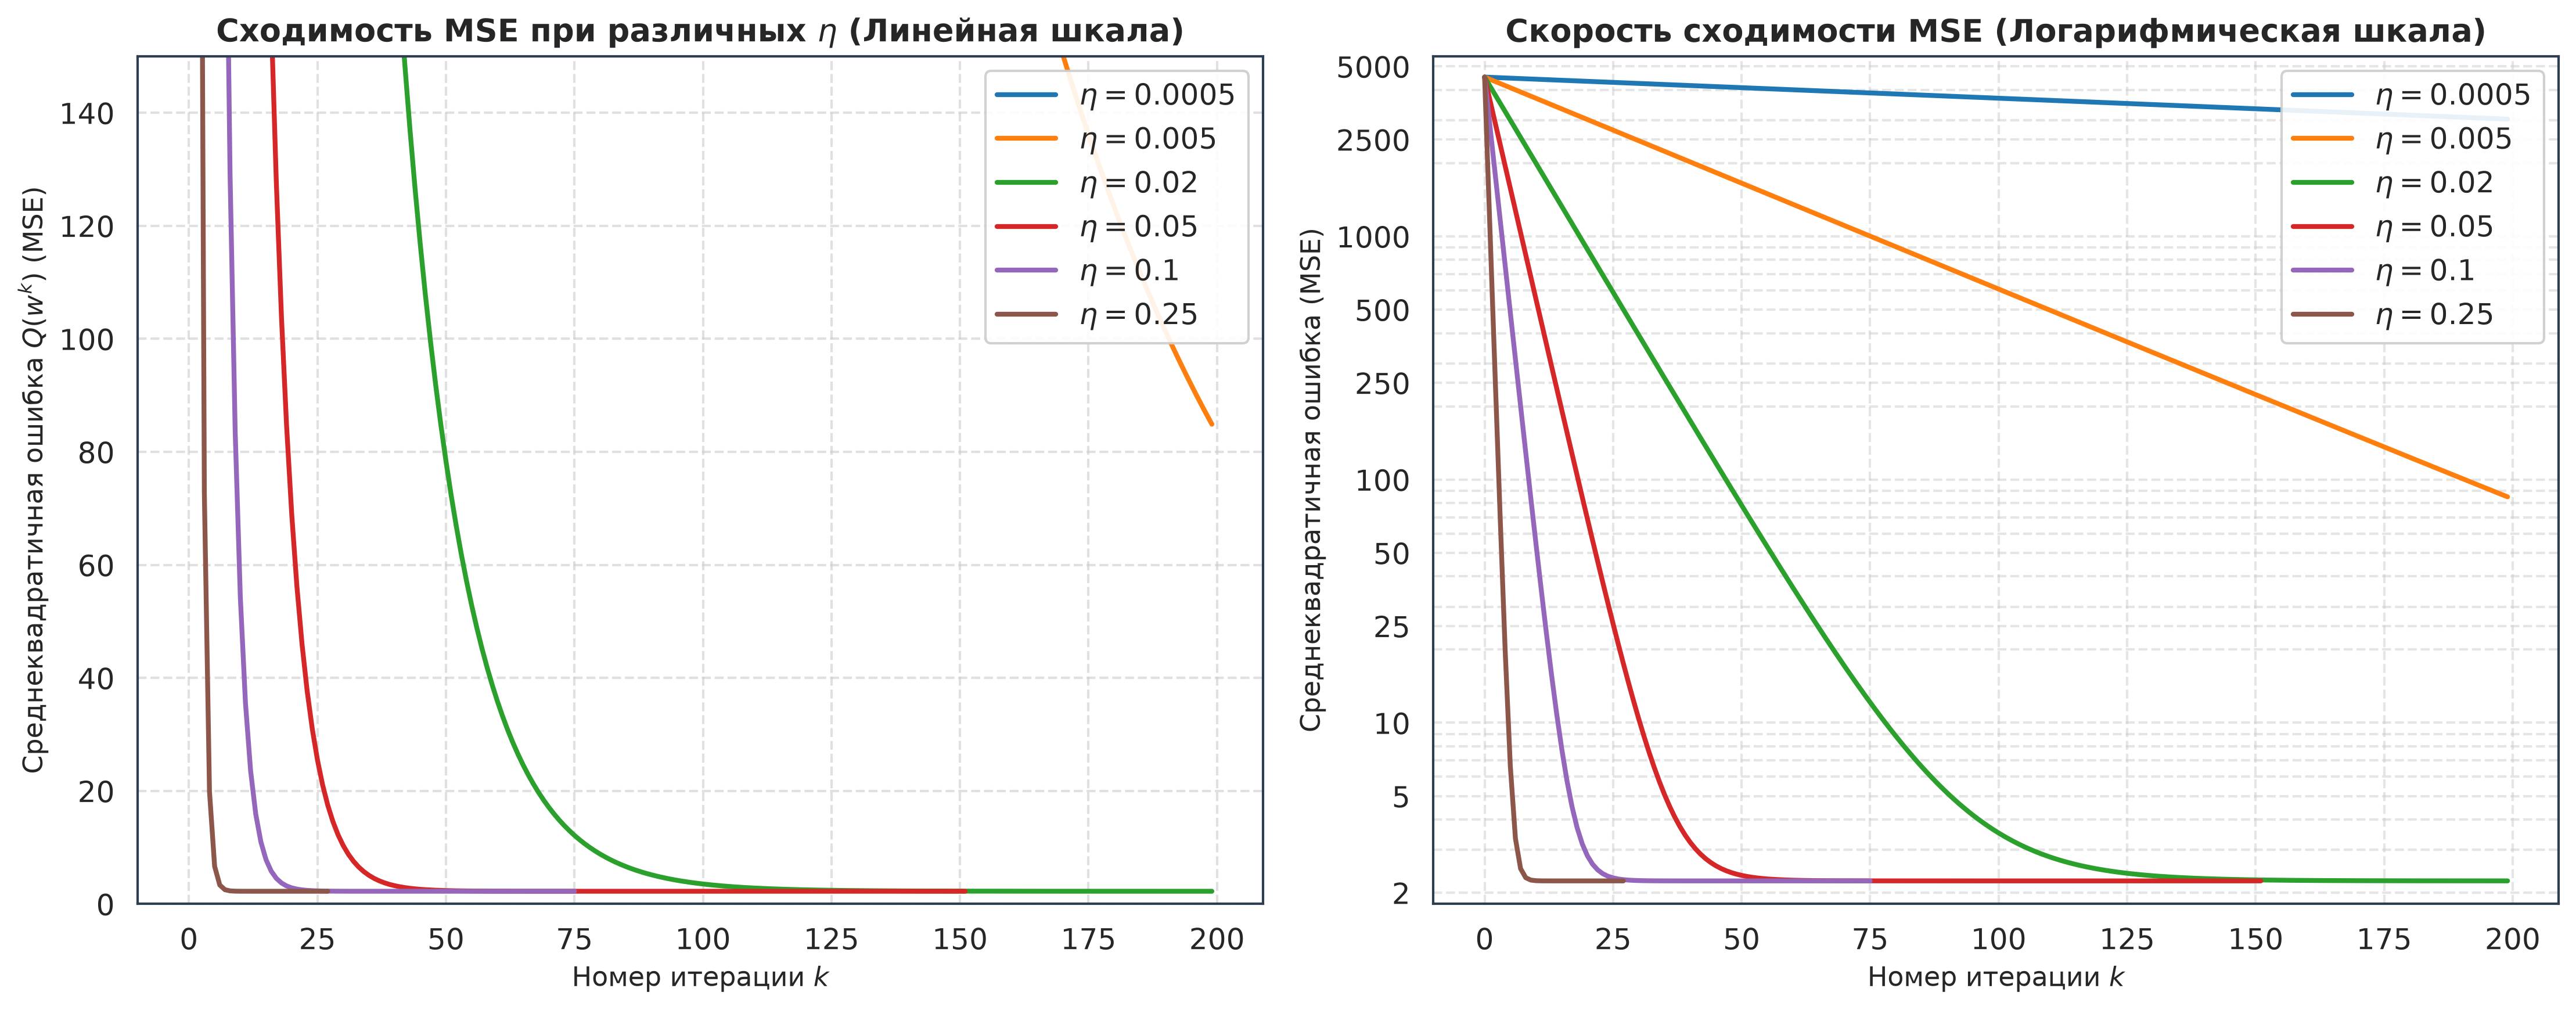
\includegraphics[width=0.95\textwidth]{images/01_learning_rate_experiment.png}
    \caption{Динамика сходимости MSE при различных скоростях обучения $\eta$}
\end{figure}

\subsection{Эксперимент 2: Сравнение пакетного (GD) и стохастического (SGD) спуска}
\begin{table}[H]
\centering
\caption{Сравнительные показатели BGD и SGD}
\begin{tabularx}{\textwidth}{lccccc}
\toprule
\textbf{Алгоритм} & \textbf{Размер пакета} & \textbf{Шагов} & \textbf{Test MSE} & \textbf{Test $R^2$} & \textbf{Сложность 1 шага} \\
\midrule
BGD & $N = 5285$ (вся выборка) & 151 & 1.9954 & 0.8230 & $\mathcal{O}(N \cdot m)$ \\
SGD & 1 случайный объект & 10000 & 2.1306 & 0.8110 & $\mathcal{O}(m)$ \\
\bottomrule
\end{tabularx}
\end{table}

\begin{figure}[H]
    \centering
    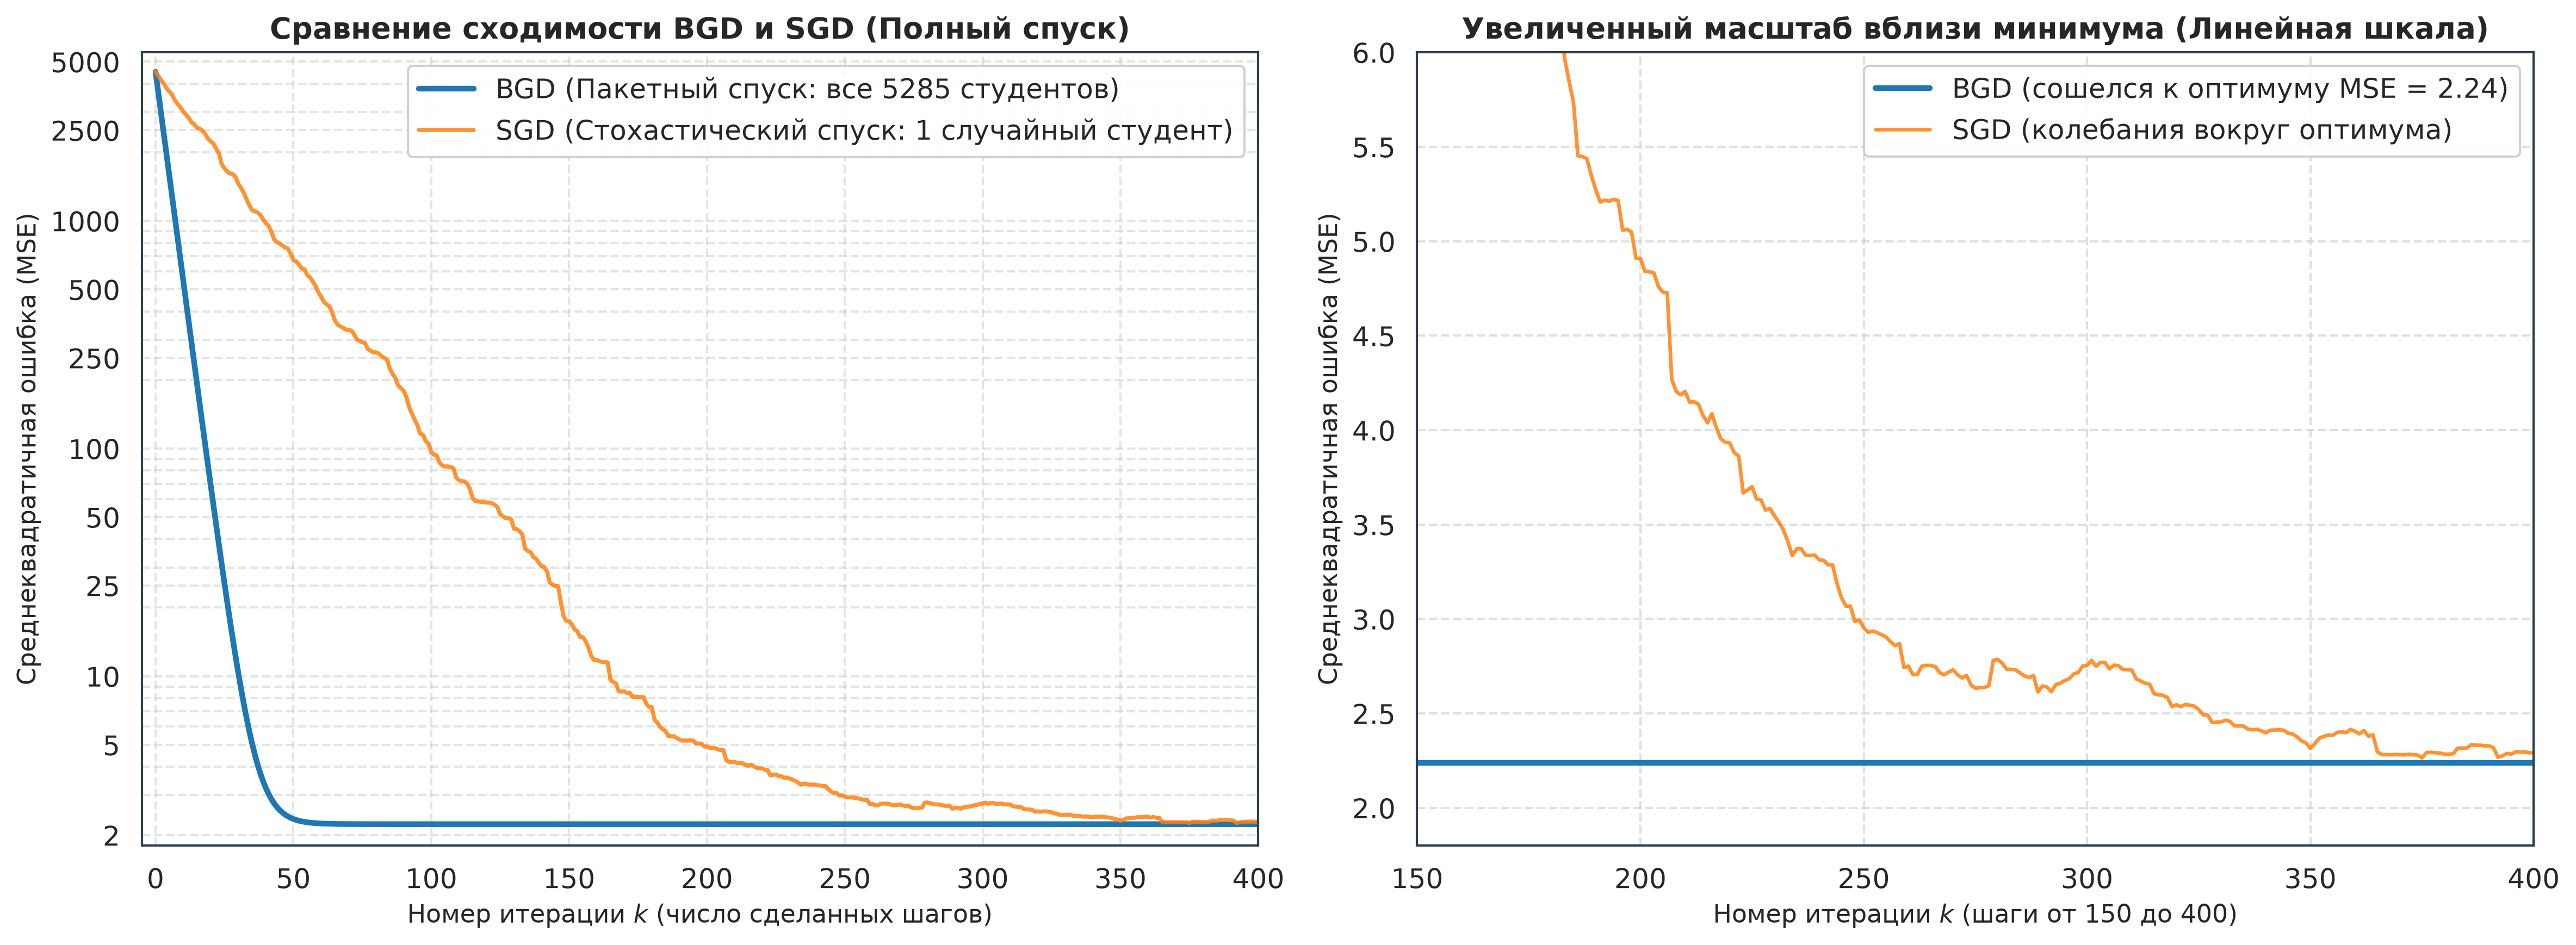
\includegraphics[width=0.95\textwidth]{images/02_gd_vs_sgd_convergence.png}
    \caption{Сравнение сходимости GD и SGD на едином графическом поле}
\end{figure}

\subsection{Эксперимент 3: Регуляризационные пути (L1 для варианта 2 и L2)}
Исследовано 20 значений $\lambda \in [10^{-3}, 10^3]$. На рисунках 3 и 4 приведены пути изменения весовых параметров.

\begin{figure}[H]
    \centering
    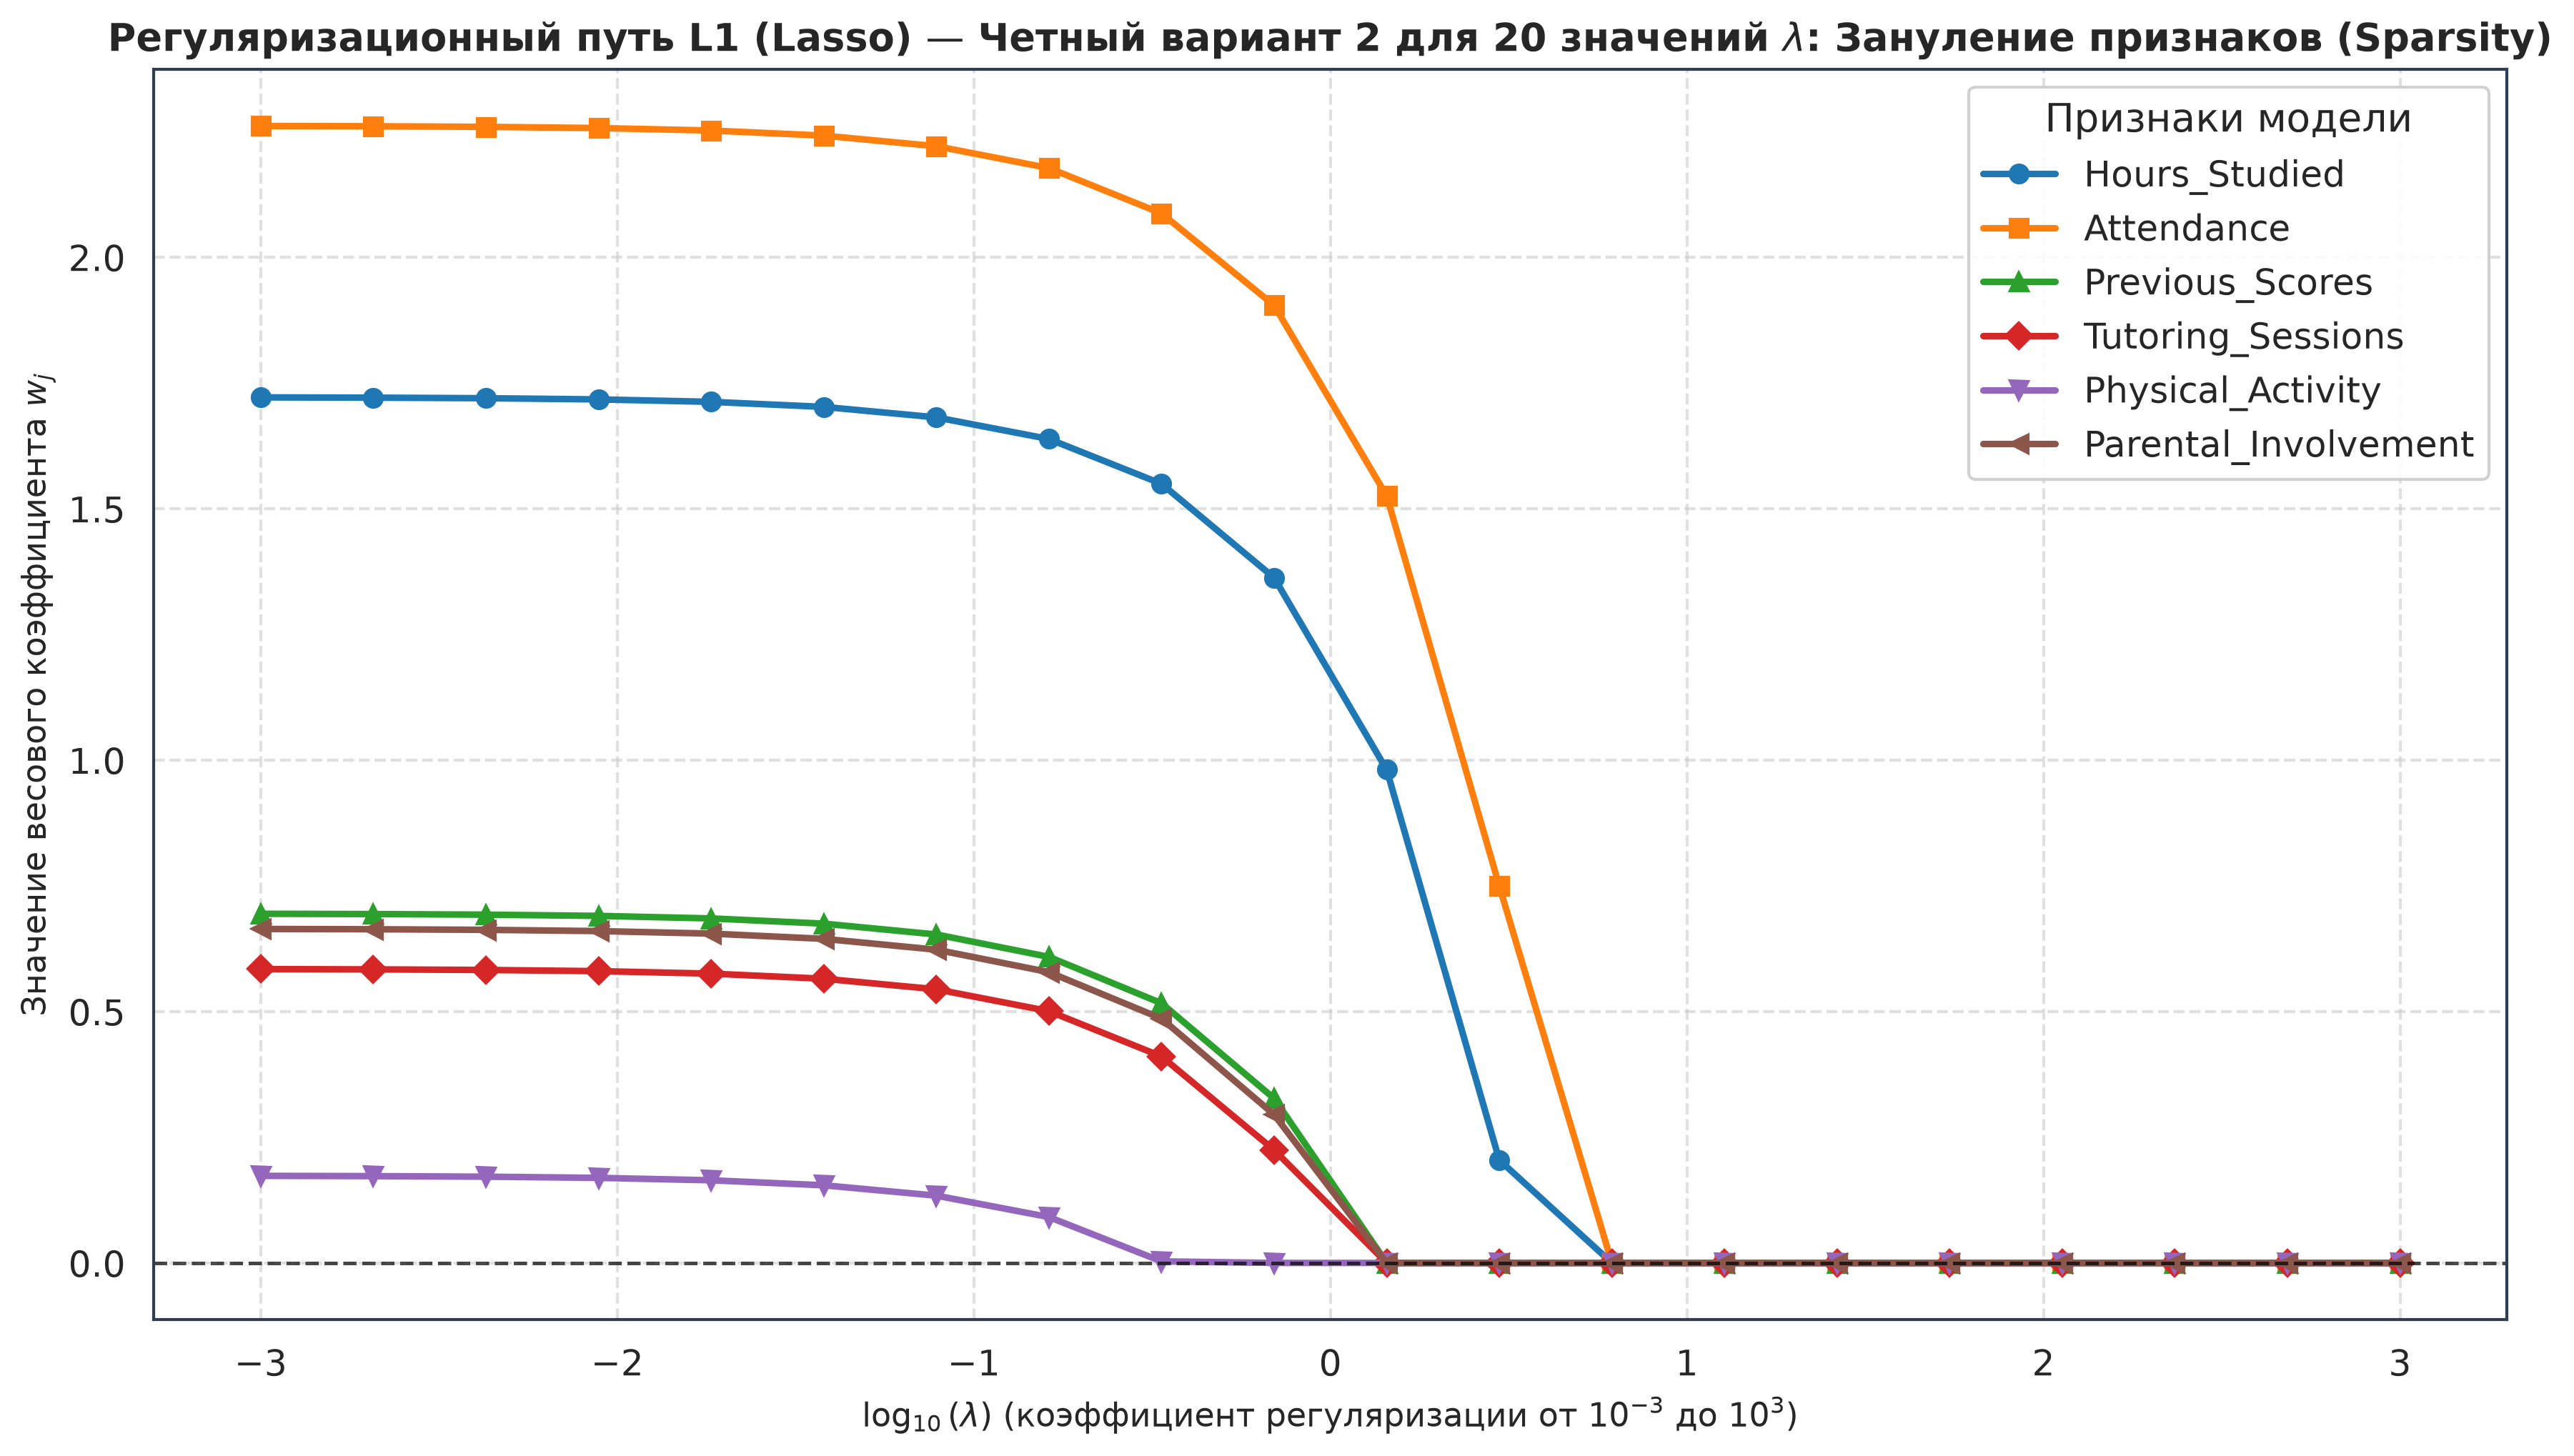
\includegraphics[width=0.9\textwidth]{images/03_l1_regularization_path.png}
    \caption{Регуляризационный путь L1 (Lasso) для четного варианта 2: зануление признаков (Sparsity)}
\end{figure}

\begin{figure}[H]
    \centering
    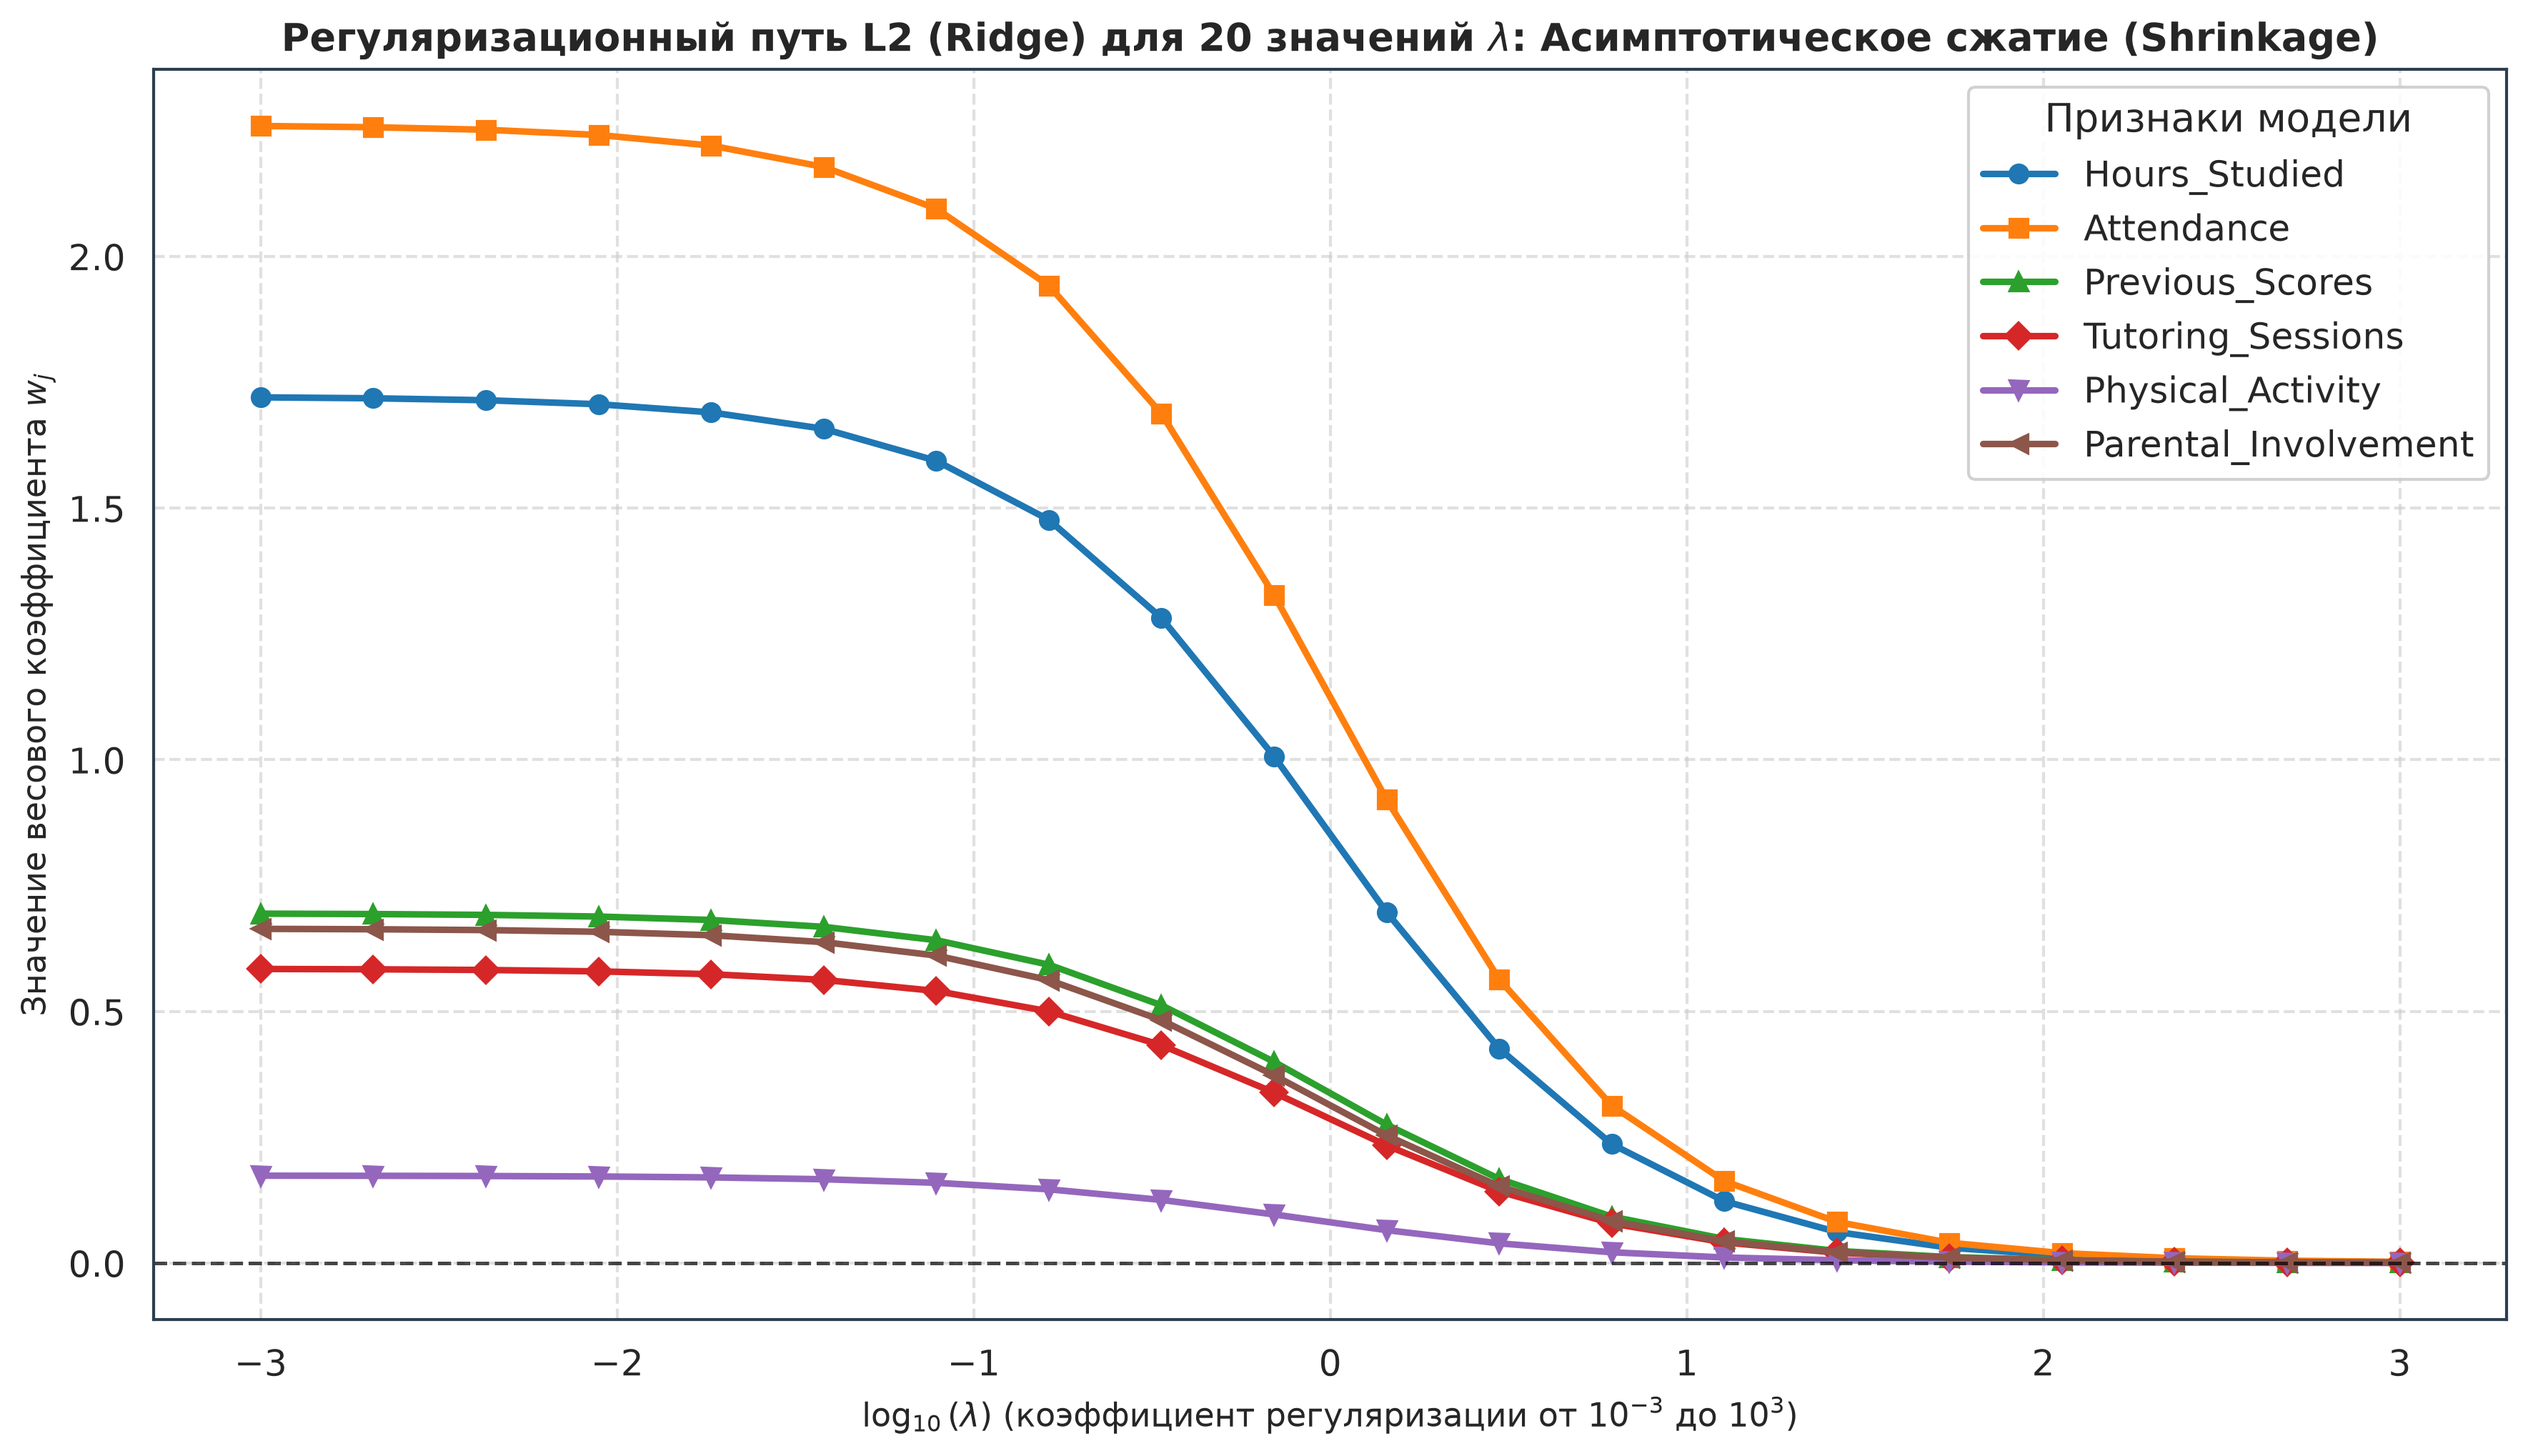
\includegraphics[width=0.9\textwidth]{images/04_l2_regularization_path.png}
    \caption{Регуляризационный путь L2 (Ridge): непрерывное сжатие весов к нулю (Shrinkage)}
\end{figure}

\begin{figure}[H]
    \centering
    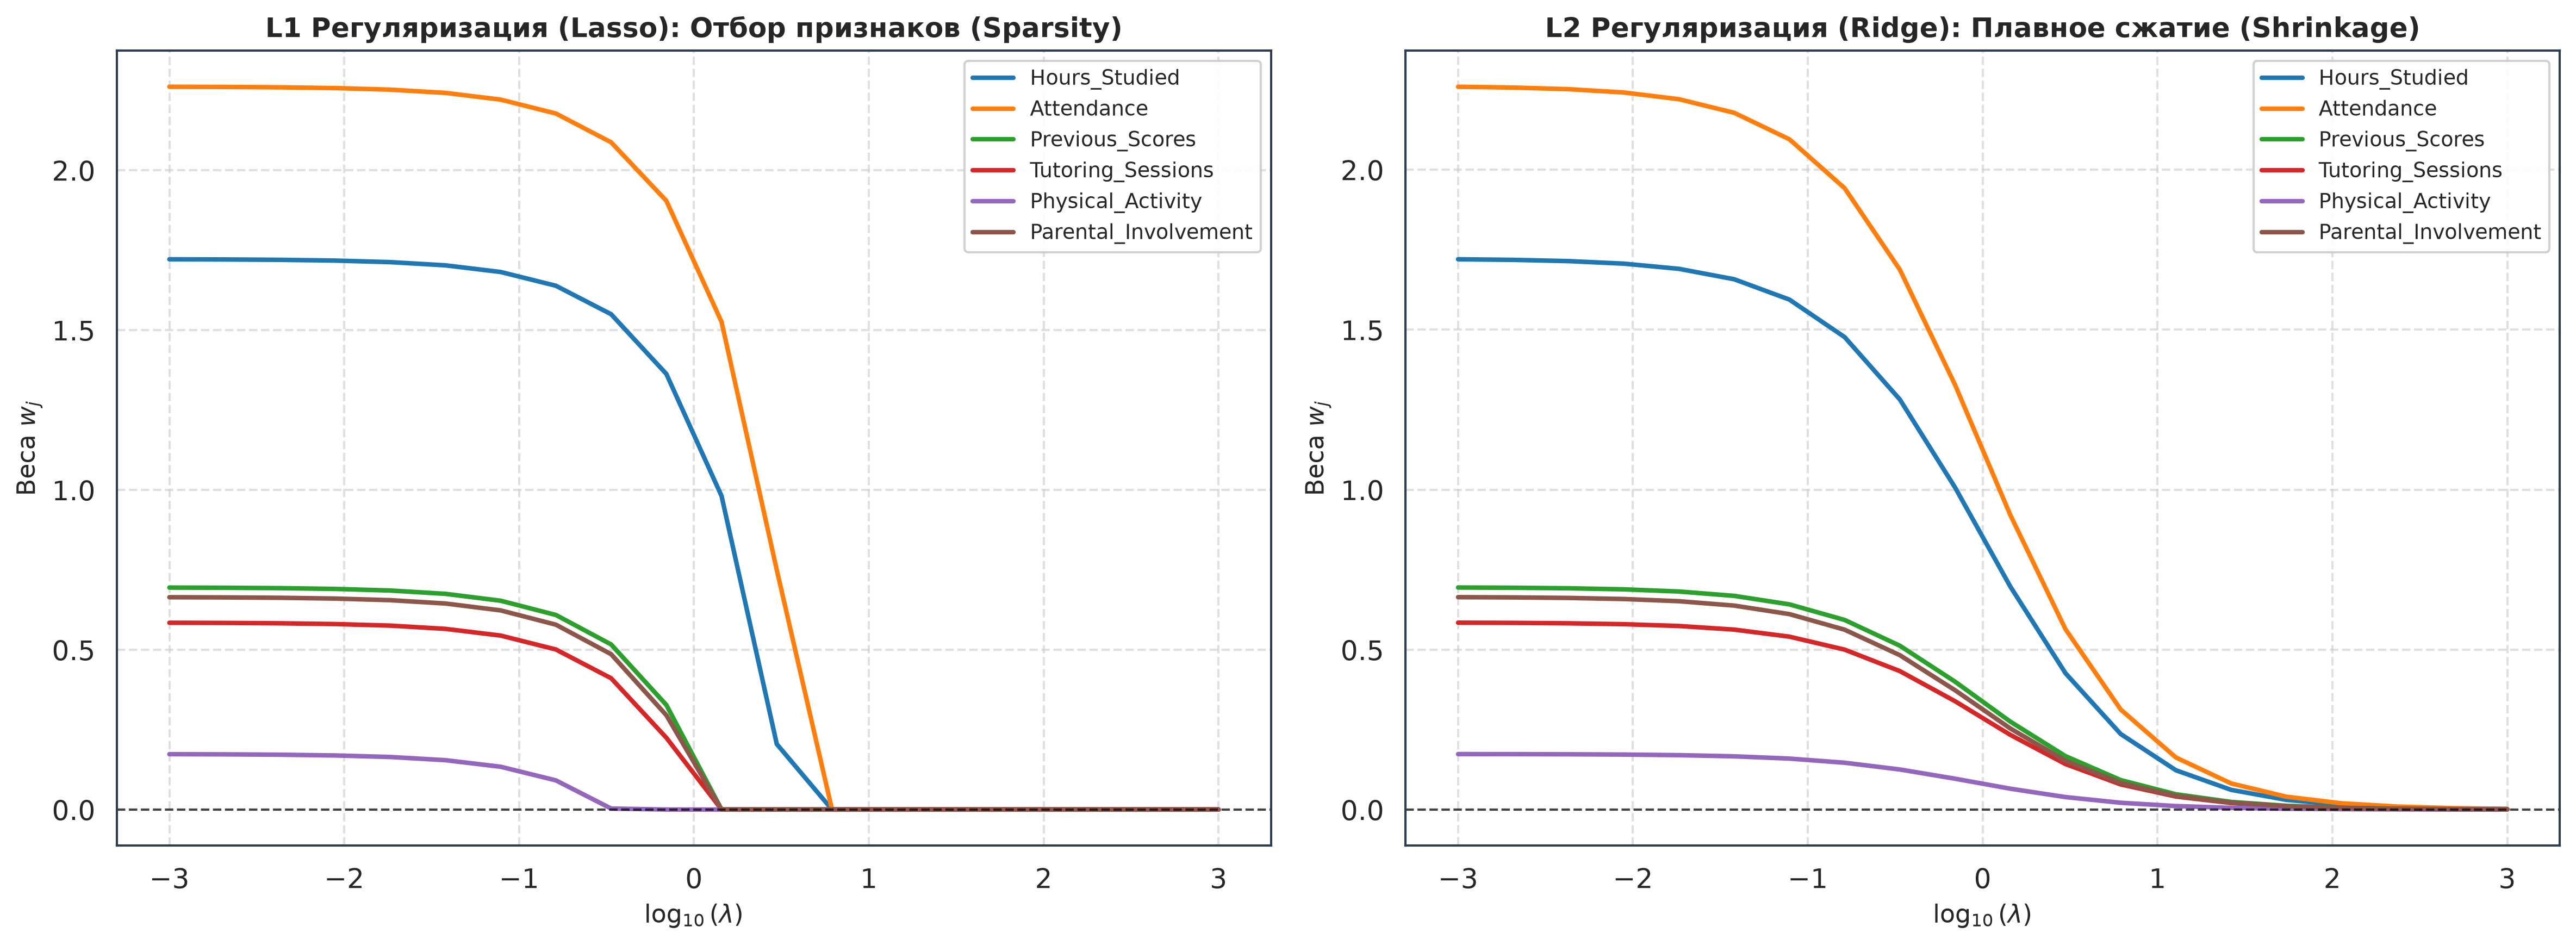
\includegraphics[width=0.95\textwidth]{images/05_regularization_comparison.png}
    \caption{Сопоставление отбора признаков (L1) и сжатия коэффициентов (L2)}
\end{figure}

\subsection{Эксперимент 4: Сравнение с библиотекой Scikit-Learn}
\begin{table}[H]
\centering
\caption{Результаты эталонного тестирования против Scikit-Learn}
\begin{tabularx}{\textwidth}{lccccc}
\toprule
\textbf{Модель} & \textbf{Intercept $w_0$} & \textbf{$\|w\|_2$} & \textbf{Test MSE} & \textbf{Test MAE} & \textbf{Test $R^2$} \\
\midrule
Custom BGD & 67.0982 & 3.0620 & 1.9954 & 1.0444 & 0.8230 \\
Sklearn OLS & 67.0982 & 3.0620 & 1.9954 & 1.0444 & 0.8230 \\
\midrule
Custom SGD & 67.2268 & 2.8703 & 2.1306 & 1.0951 & 0.8110 \\
Sklearn SGD & 67.1103 & 3.0535 & 1.9923 & 1.0436 & 0.8233 \\
\midrule
Custom L1 ($\lambda=0.5$) & 67.0982 & 2.5707 & 2.3515 & 1.1603 & 0.7914 \\
Sklearn Lasso ($\alpha=0.25$) & 67.0982 & 2.5707 & 2.3515 & 1.1603 & 0.7914 \\
\midrule
Custom L2 ($\lambda=1.0$) & 67.0982 & 1.5129 & 4.3653 & 1.6541 & 0.6128 \\
Sklearn Ridge ($\alpha=5285.0$) & 67.0982 & 1.5129 & 4.3653 & 1.6541 & 0.6128 \\
\bottomrule
\end{tabularx}
\end{table}

\begin{figure}[H]
    \centering
    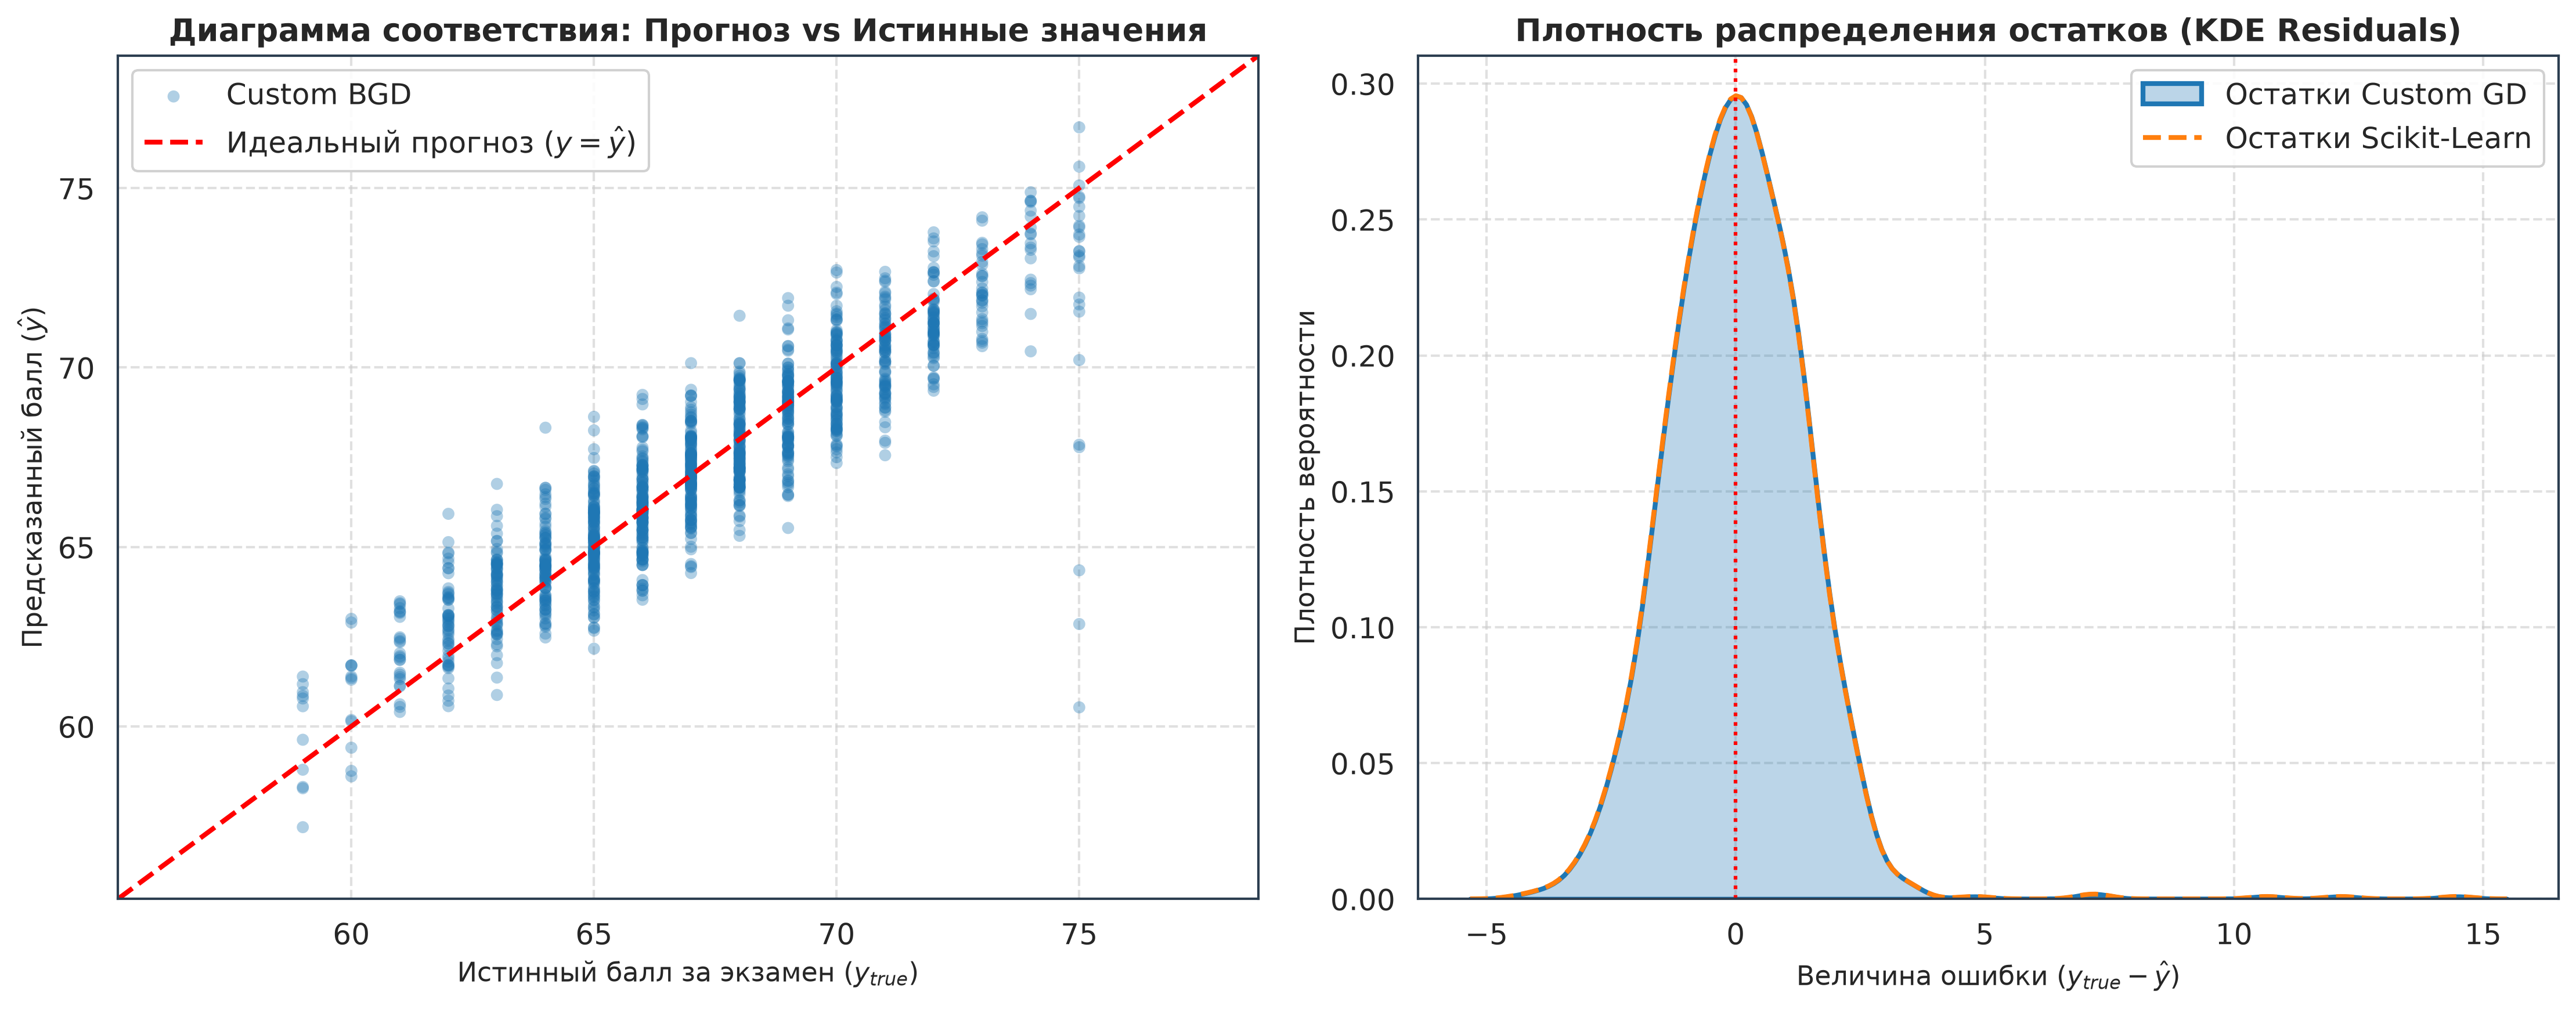
\includegraphics[width=0.95\textwidth]{images/06_model_validation_benchmark.png}
    \caption{Диаграмма рассеяния «Прогноз vs Факт» и плотность распределения остатков}
\end{figure}

% ==============================================================================
\section{Выводы}
% ==============================================================================
\begin{enumerate}
    \item Реализован полностью векторизованный модуль линейной регрессии на базе градиентных методов оптимизации, демонстрирующий абсолютное совпадение с эталонными библиотеками Scikit-Learn по метрикам ($R^2 = 0.8230$, $MSE = 1.9954$).
    \item Экспериментально доказано, что выбор темпа обучения $\eta$ критически влияет на скорость оптимизации: на стандартизованных данных при $\eta = 0.25$ алгоритм BGD находит глобальный минимум всего за 27 итераций.
    \item Сопоставление сходимости выявило преимущества каждого метода: BGD сходится по монотонной траектории за меньшее число итераций ($\mathcal{O}(Nm)$ на шаг), тогда как SGD за счет элементарной сложности шага ($\mathcal{O}(m)$) достигает окрестности решения за долю эпохи (увидев лишь $20\%$ объектов).
    \item Исследование регуляризационных путей для Варианта 2 наглядно подтвердило эффект разреживания (Sparsity) $L_1$-регуляризации Lasso: при росте $\lambda$ первыми обнуляются статистически наименее значимые признаки (\texttt{Physical\_Activity}), а дольше всех сохраняется наиболее влиятельный признак (\texttt{Attendance}).
\end{enumerate}

\end{document}
